We use a simple example to introduce the semantics of the CWP and BPMN models. The example describes the well-known and easily-understandable process of a face-to-face private sale transaction. Private sale transactions are characterized by two parties, the buyer and the seller. In order for the sale to take place, terms and price must be agreed upon by both parties. Then, payment must be exchanged from the buyer to the seller and a product or service must be exchanged from the seller to the buyer. To further simplify the example, this CWP uses labels indicating that the product being sold is a backpack. Aside from the labels, there is nothing preventing this CWP to be used in other private sale transactions.

The CWP accomplishes two things. First, it introduces an object state composed of a set of variables. Second, it uses that object state in a transition system that defines a problem or proposed work. The variables and possible values in the object state are inferred from the set of logical conditions attached to the edges of the transition system.

This CWP's transition system, shown in \figref{fig:purchase_cwp}, has five states, of which two are goal states. The workflow, shown in \figref{fig:face2face_error_bpmn} is responsible for transforming the object state to the goal state using only valid transitions as defined by the CWP. This example of a face-to-face purchase will be called "Face2Face" throughout the paper. The first state is in the top left corner, where the purchase has been initialized. Next, there is a state near the center encompassing terms and price negotiations. There are then states for either the purchase failing near the bottom or being agreed upon in the top right. Finally, there is a state at the bottom right that indicates the ownerships of the item and payment have switched parties.

\begin{figure*}[t]
  \begin{center}
    \begin{tabular}{c}
        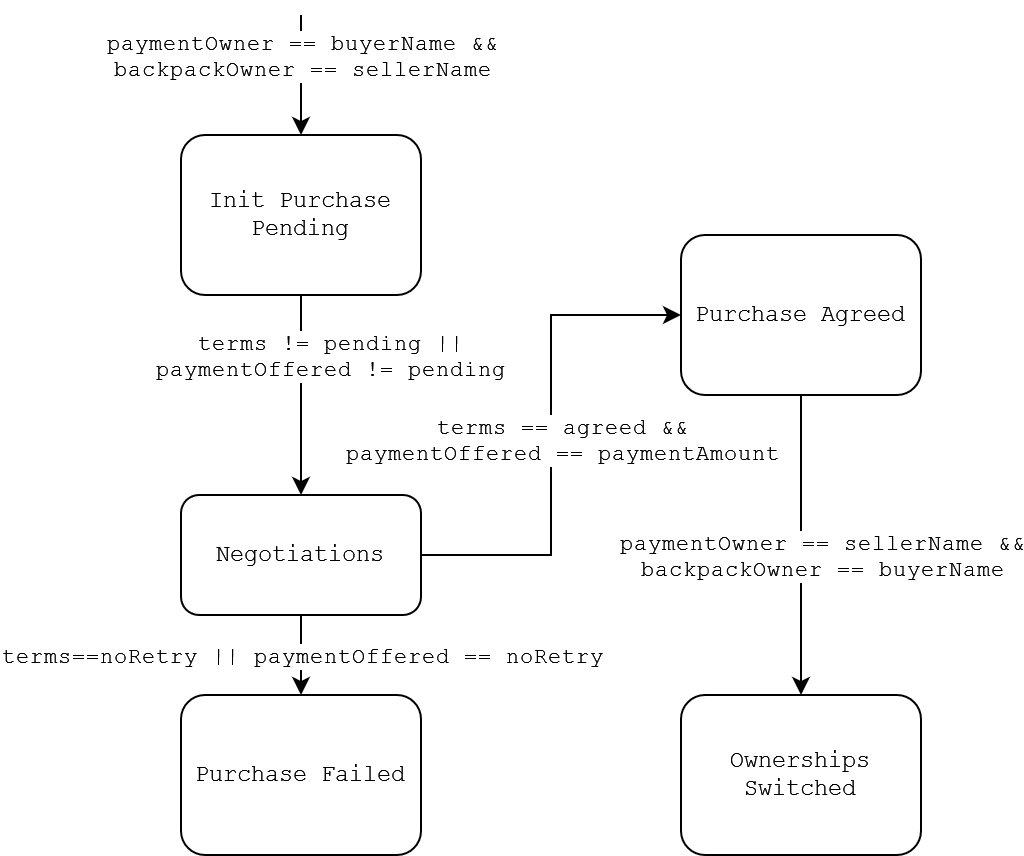
\includegraphics[width=\textwidth]{paper/figs/CWP/purchase_CWP.png}
    \end{tabular}
  \end{center}
\caption{CWP state diagram for a purchase with negotiations}
\label{fig:purchase_cwp}
\end{figure*}


\begin{figure*}[t]
  \begin{center}
    \begin{tabular}{c}
        \includesvg[inkscapeformat=png, width=\textwidth]{../figs/BPMN/face2face_May_5_2023_error_workflow.svg}
    \end{tabular}
  \end{center}
\caption{Erroneous BPMN workflow for a face-to-face purchase with negotiations.}
\label{fig:face2face_error_bpmn}
\end{figure*}

The BPMN workflow for the Face2Face example is shown in \figref{fig:face2face_error_bpmn}. To fascilitate understanding of the semantics of the diagram, I employ a token, a concept used by the creators of BPMN on page 25 of the BPMN specification \cite{BPMNSpecification}. In the authors' words, a token "will traverse the Sequence Flows and pass through the elements in the Process. [It] is a theoretical concept that is used as an aid to define the behavior of a Process that is being performed. The behavior of Process elements can be defined by describing how they interact with a token as it “traverses” the structure of the Process."

The Face2Face BPMN workflow begins on the left with the start event "Start7." The token then flows through to task one, where the buyer and seller meet. Then, the token flows to gateway "XOR1", which acts as a joining gateway for a looping structure encountered later. Then, the token flows to task 2, where negotiations happen for both price and terms of the purchase. Next, an exclusive OR gateway branches the flow based on whether or not the negotiations were successful. If they were, and both parties agreed on price and terms, the token can continue to task 6, where they shake hands, and then further on to "both1," a parallel gateway. Here, the token is duplicated and flows down both outgoing paths to tasks 7a and 7b where the payment and the backpack are exchanged. Another parallel gateway, "end both1," waits for both tokens to arrive before sending a token through to "Purchase Completed," a successful end event. If negotiations were unsuccessful initially, the XOR gateway sends the token back to either task 4, task 5, or XOR1, depending on whether price, terms, or both were unsuccessful. Renegoatiations are then repeated until the parties either agree on both terms and price, or they decide not to retry. If they decide not to retry, the token flows to the unsuccessful end event, "Purchase Failed."

\bryce{I am not sure if I should be explaining the injected error and the resulting fix here or later, in the evaluation section.}

Code snippets used throughout the paper are in reference to Face2Face.

\begin{figure*}[t]
  \begin{center}
    \begin{tabular}{c}
        \includesvg[inkscapeformat=png, width=\textwidth]{../figs/BPMN/face2face_May_5_2023_workflow.svg}
    \end{tabular}
  \end{center}
\caption{BPMN workflow for a face-to-face purchase with negotiations}
\label{fig:face2face_bpmn}
\end{figure*}

\begin{figure*}[t]
  \begin{center}
    \begin{tabular}{c}
        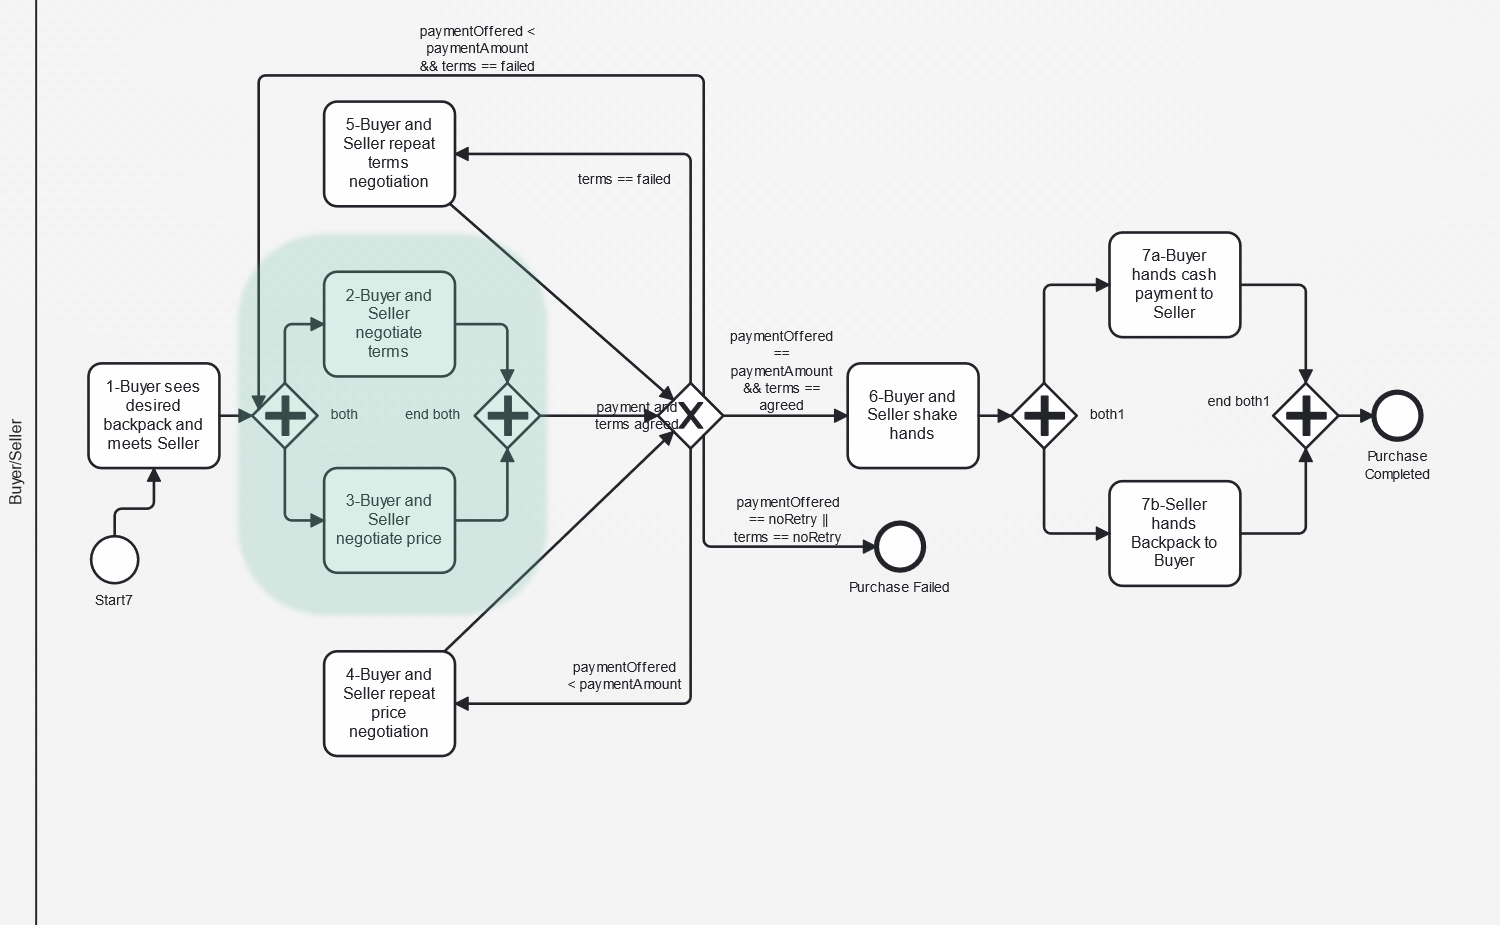
\includegraphics[width=\textwidth]{paper/figs/BPMN/face2face_May_5_2023_workflow_fixed.png}
    \end{tabular}
  \end{center}
\caption{Fixed BPMN workflow for a face-to-face purchase with negotiations}
\label{fig:face2face_bpmn_fixed}
\end{figure*}